\subsection{Depthwise Separable Convolution}  \label{subs:dsc}
\acrfull{dsc} is first introduced by \textcite{sifre_ecole_2014}. According to \textcite{chollet_xception_2017}, "\textit{A depthwise separable convolution consists in a \textbf{depthwise convolution}, i.e. a spatial convolution performed independently over each channel of an input, followed by a \textbf{pointwise convolution}, i.e. a 1x1 convolution, projecting the channel's output by the depthwise convolution onto a new channel space}".

As said above, the \acrshort{dsc} is composed of a depthwise convolution and a pointwise convolution. An illustration of the operation is shown in Figure \ref{fig:dsc}. This alternative form of convolution has been developed to reduce the the arithmetic operations, in exchange for a limited loss of accuracy \cite{liu_fpga-based_2019}. As a result, the \acrshort{dsc} has fewer parameters and faster inference with respect to the standard convolution. The reduction factors on weight and operation are calculated in Equation \eqref{eq:descopred} and Equation \eqref{eq:descwgred}, where $F_{*}$ are the factors of reduction, $W_{sc}$ and $O_{sc}$ are the weights and operations required for a standard convolution, and $W_{dsc}$ and $O_{dsc}$ are the weights and operations required for a \acrshort{dsc}.
%
\begin{equation}
    F_w = \frac{W_{dsc}}{W_{sc}} =
    \frac{N_{kx} \times N_{ky} \times N_{if} + N_{if} \times N_{of}}{N_{kx} \times N_{ky} \times N_{if} \times N_{of}} =
    \frac{1}{N_{of}} + \frac{1}{N_{kx} \times N_{ky}}
    \label{eq:descopred}
\end{equation}
\begin{equation}
    \begin{split}
        F_o &= \frac{O_{dsc}}{O_{sc}} = \frac{N_{kx} \times N_{ky} \times N_{if} \times N_{ox} \times N_{oy} + N_{if} \times N_{of} \times N_{ox} \times N_{oy}}{N_{kx} \times N_{ky} \times N_{if} \times N_{of} \times N_{ox} \times N_{oy}} \\
        &= \frac{1}{N_{of}} + \frac{1}{N_{kx} \times N_{ky}}
    \end{split}
    \label{eq:descwgred}
\end{equation}

Using Equation \eqref{eq:descopred} and Equation \eqref{eq:descwgred} and $3 \times 3$ kernels, the reduction of computation and parameters with respect to the standard convolution is about 9 times \cite{zhang_channel_2019}.
%
\begin{figure}
    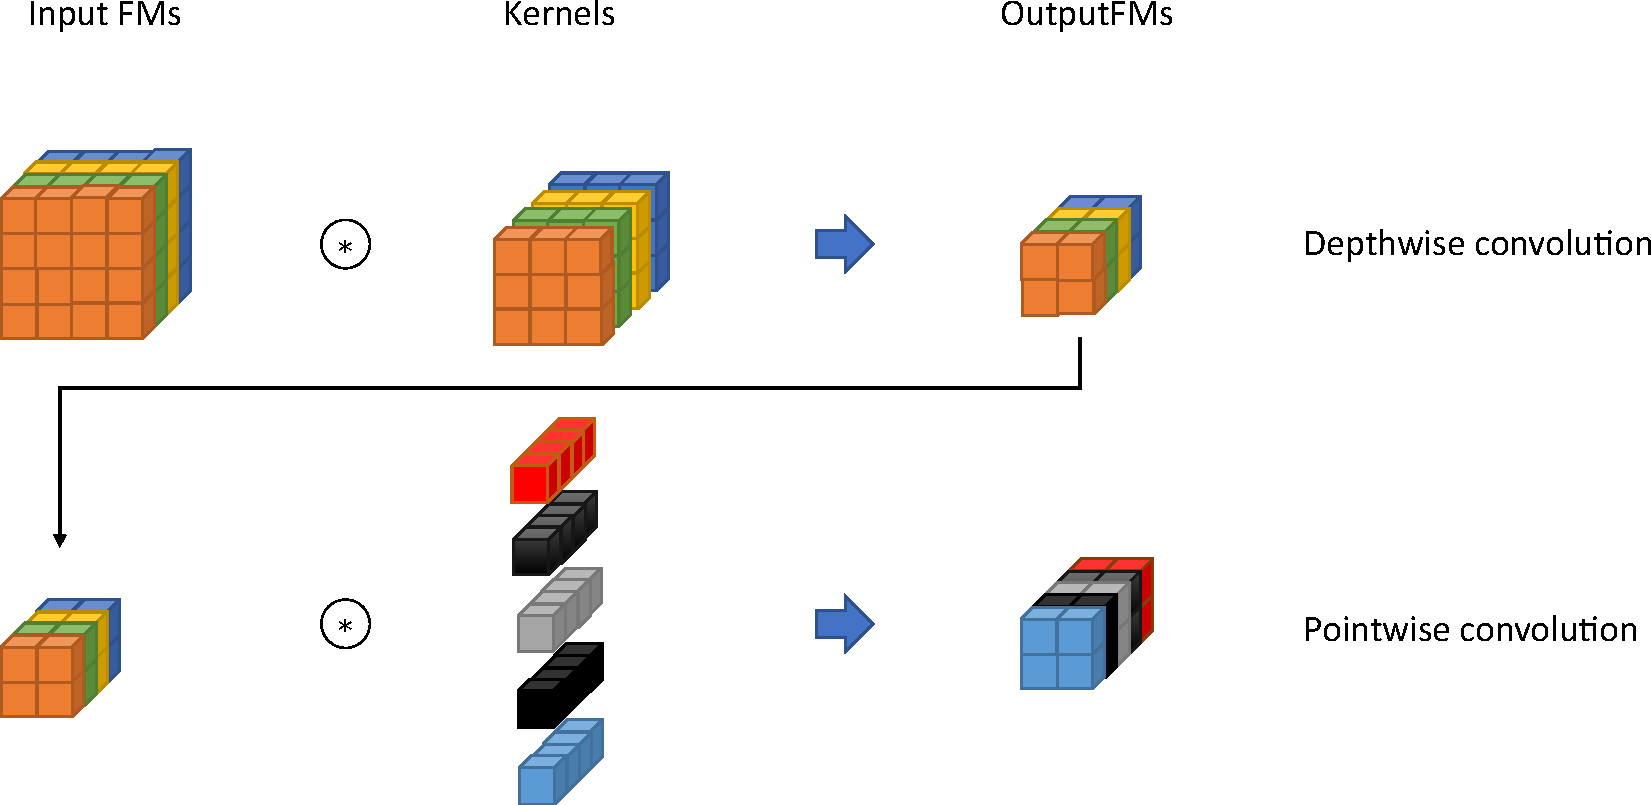
\includegraphics[width=\textwidth]{dsc.pdf}
    \caption{Depthwise Separable Convolution}
    \label{fig:dsc}
\end{figure}
